\documentclass[]{beamer}
\mode<presentation>
{
  \usetheme{Warsaw}
  \definecolor{mcgarnet}{rgb}{0.38, 0, 0.08}
  \definecolor{mcgray}{rgb}{0.6, 0.6, 0.6}
  \setbeamercolor{structure}{fg=mcgarnet,bg=mcgray}
  %\setbeamercovered{transparent}
}


\usepackage[english]{babel}
\usepackage[latin1]{inputenc}
\usepackage{times}
\usepackage[T1]{fontenc}
\usepackage{tikz}
\usepackage{graphicx}
\usepackage{adjustbox}
\usepackage{fancyvrb}

\newcommand{\imagesource}[1]{{\centering\hfill\break\hbox{\scriptsize Image Source:\thinspace{\small\itshape #1}}\par}}

\title{02 - C++ Design and Thinking}


\author{Dr. Robert Lowe\\}

\institute[Maryville College] % (optional, but mostly needed)
{
  Division of Mathematics and Computer Science\\
  Maryville College
}

\date[]{}
\subject{}

\pgfdeclareimage[height=0.5cm]{university-logo}{images/Maryville-College}
\logo{\pgfuseimage{university-logo}}



\AtBeginSection[]
{
  \begin{frame}<beamer>{Outline}
    \tableofcontents[currentsection]
  \end{frame}
}


\begin{document}

\begin{frame}
  \titlepage
\end{frame}

\begin{frame}{Outline}
  \tableofcontents
\end{frame}


% Structuring a talk is a difficult task and the following structure
% may not be suitable. Here are some rules that apply for this
% solution: 

% - Exactly two or three sections (other than the summary).
% - At *most* three subsections per section.
% - Talk about 30s to 2min per frame. So there should be between about
%   15 and 30 frames, all told.

% - A conference audience is likely to know very little of what you
%   are going to talk about. So *simplify*!
% - In a 20min talk, getting the main ideas across is hard
%   enough. Leave out details, even if it means being less precise than
%   you think necessary.
% - If you omit details that are vital to the proof/implementation,
%   just say so once. Everybody will be happy with that.
\section{Loops}

\begin{frame}[fragile]{While Loop}
  \begin{columns}
    \column{0.5\textwidth}

    \begin{block}{While Loop Syntax}
      \verb!while(! \textit{condition} \verb!)! 
      \newline\verb!    ! \textit{statement/block}
    \end{block}
    
    \vspace{0.5cm}

    \begin{itemize}[<+(1)->]
      \item If the \textit{condition} is true, the loop body is executed.
      \item After the loop body executes, the process begins again.
      \item How many times will the loop body execute?
      \begin{itemize}
          \item Zero or more times!
      \end{itemize}
    \end{itemize}

    \column{0.5\textwidth}
    \begin{center}
      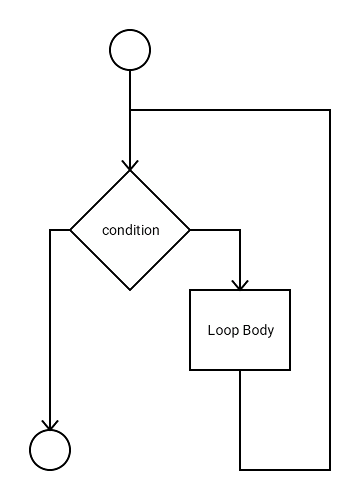
\includegraphics[width=0.8\textwidth]{images/while}
    \end{center}
  \end{columns}
\end{frame}

\begin{frame}[fragile]{Do..While Loop}
  \begin{columns}
    \column{0.5\textwidth}

    \begin{block}{While Loop Syntax}
      \verb!do! 
      \newline\verb!    ! \textit{statement/block}
      \newline\verb!while(! \textit{condition} \verb!);! 
    \end{block}
    
    \vspace{0.3cm}

    \begin{itemize}[<+(1)->]
        \item The \texttt{do..while} loop is called the postcondition
        loop.
        \item The condition is checked after the loop body.
        \item Executes 1 or more times.
        \item Commonly used with input validation and menus.
    \end{itemize}

    \column{0.5\textwidth}
    \begin{center}
      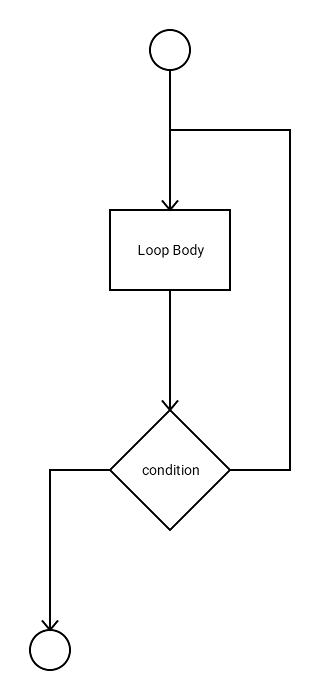
\includegraphics[height=0.9\textheight]{images/do-while}
    \end{center}
  \end{columns}
\end{frame}

\begin{frame}[fragile]{For Loop}
\begin{columns}
    \column{0.6\textwidth}
    \begin{block}{The For Loop}<2->
        \verb!for(! \textit{initialize}; \textit{condition}; \textit{update}\verb!) {!
        \newline\verb!    !\textit{loop body}
        \newline\verb!}!
    \end{block}

    \begin{block}{Example: Count to 10}<3->
        \verb!for(num=0; num <= 10; num++)!
        \newline\verb!{!
        \newline\verb!    cout << num << endl;!
        \newline\verb!}!
    \end{block}

    \column{0.4\textwidth}
    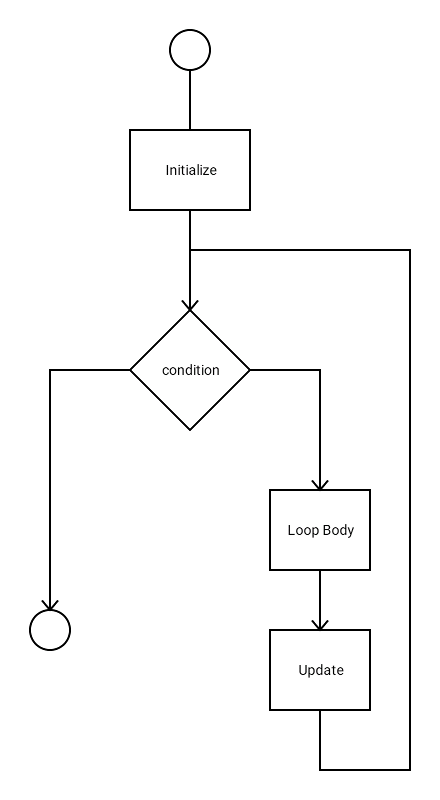
\includegraphics[width=0.9\textwidth]{images/for}
\end{columns}
\end{frame}

\section{Functions}
\begin{frame}{The Problem}
\begin{columns}
    \column{0.7\textwidth}
    \begin{itemize}[<+->]
        \item Thus far, all known software is written by humans.
        \item The human race is a member of the hominidae family.
        \item We are apes.
        \item We are the most successful ape.
        \item We are still apes, nonetheless.  
        \item We can hold about seven ideas in our heads at once.
        \item This is insufficient for almost all useful programming
            tasks.
    \end{itemize}

    \column{0.3\textwidth}
        \begin{center}
            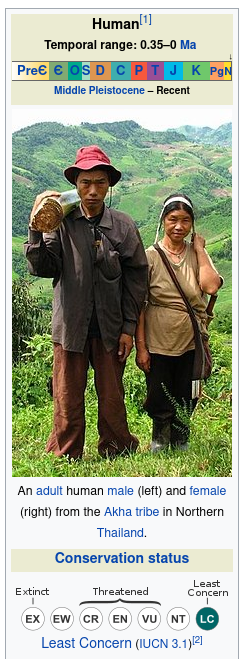
\includegraphics[height=0.75\textheight]{images/human}
            \newline
            {\tiny Source: wikipedia.org}
        \end{center}

\end{columns}
\end{frame}

\begin{frame}[fragile]{Function Definition}
    \begin{block}{Function Syntax}
        \texttt{\textit{return\_type} \textit{name}( \textit{parameters} )}
        \newline\texttt{\{}
        \newline\verb!    //function body!
        \newline\texttt{\}}
    \end{block}

    \begin{itemize}[<+(2)->]
        \item A function is a block of code that can be called
            multiple times. 
        \item A function's signature consists of the following:
        \begin{description}
            \item[return type] This is the type of value the function
                evaluates to when it is used in an expression.
            \item[name] The identifier which names the function.
            \item[parameters] The local variables which receive the
                arguments of the function.
        \end{description}
    \end{itemize}
\end{frame}

\begin{frame}[fragile]{Function Prototypes}
    \begin{itemize}[<+->]
        \item Function prototypes allow you to declare a function
            before it is defined.
        \item This is a sort of ``contract'' between you and the
            compiler.
        \item This allows you to have functions in any order in the
            file.  
        \item Change the first few lines of \texttt{roman.cpp} so it
            reads as follows:
            \newline
            \newline
            \begin{BVerbatim}
#include <iostream>

using namespace std;

//function prototypes
void print_roman_numeral(int value);
            \end{BVerbatim}
    \end{itemize}
\end{frame}

\begin{frame}{Gluing it Together With Header Files}
    \begin{itemize}[<+->]
        \item A function must be declared before it can be used.
        \item Because the definitions are in a separate file, they are
            not declared in the file that contains our main function.
        \item We can solve this with prototypes.
        \item Repeating prototypes in every file is painful.
        \item Enter the header file!  
        \item A header file usually has a \texttt{.h} extension and
            contains:
            \begin{itemize}
                \item Function Prototypes
                \item Constants
                \item Type Definitions
            \end{itemize}
    \end{itemize}
\end{frame}

\section{Makefile}
\begin{frame}[fragile]{Makefile -- Explicit Recipes}
\begin{adjustbox}{max width=\textwidth, max totalheight=0.9\textheight}
\begin{BVerbatim}
sodasim: sodasim.o soda-machine.o
    g++ -o sodasim sodasim.o soda-machine.o

sodasim.o: sodasim.cpp soda-machine.h
soda-machine.o: soda-machine.cpp soda-machine.h
\end{BVerbatim}
\end{adjustbox}
\end{frame}

\begin{frame}[fragile]{Some Predefined Variables}
\begin{itemize}[<+->]
    \item The make syntax is itself a scripting language.
    \item Variables begin with dollar signs \$.  
    \item There are several pre-defined variables, the two most
        commonly used ones are:
        \begin{itemize}
            \item \verb!$@! -- The name of the target
            \item \verb!$^! -- The list of all ingredients
        \end{itemize}
    \item We could simplify the sodasim \texttt{Makefile} like so:
\begin{adjustbox}{max width=\textwidth, max totalheight=0.9\textheight}
\begin{BVerbatim}
sodasim: sodasim.o soda-machine.o
    g++ -o $@ $^

sodasim.o: sodasim.cpp soda-machine.h
soda-machine.o: soda-machine.cpp soda-machine.h
\end{BVerbatim}
\end{adjustbox}
\end{itemize}
\end{frame}

\begin{frame}[fragile]{Example Makefile -- Address Book}
\begin{adjustbox}{max width=\textwidth, max totalheight=0.9\textheight}
\begin{BVerbatim}
TARGETS=stock

#application builds
all: $(TARGETS)
stock: iofun.o main.o stock.o transaction.o portfolio.o
	g++ -o $@ $^

#object files
iofun.o: iofun.h iofun.cpp
main.o: main.cpp iofun.h stock.h transaction.h portfolio.h
stock.o: stock.h stock.cpp
transction.o: transaction.cpp transaction.h
portfolio.o: portfolio.cpp portfolio.h


#delete all binaries
clean:
	rm -f *.o $(TARGETS)
\end{BVerbatim}
\end{adjustbox}
\end{frame}

\section{Lab Assignment}
\begin{frame}[fragile]{Programming Project 5.9}
\begin{block}{Programming Project 5.9 from Big C++}
Write a program that, given a month and year, prints a calendar, such as
\begin{verbatim}
           June 2016
     Su Mo Tu We Th Fr Sa
               1  2  3  4
      5  6  7  8  9 10 11
     12 13 14 15 16 17 18
     19 20 21 22 23 24 25
     26 27 28 29 30
\end{verbatim}
Make a helper function to print the header and a helper function to print each
row.
\end{block}
\end{frame}

\end{document}


